\documentclass[12pt]{article}

\usepackage{background}     % Defining text colours.
\usepackage{caption}        % Caption without "Figure" at the start of it.
\usepackage{enumitem}       % Better enumeration
\usepackage{fancyhdr}       % Headers and footers.
\usepackage[none]{hyphenat} % No hyphenation
\usepackage{lastpage}       % To determine the last page of the document for
                            % the header.
\usepackage{parskip}        % Removes indentations from paragraphs.
\usepackage{wrapfig}        % Figures beside text.
\usepackage{xcolor}         % Coloured text.

% Setting dimensions
\usepackage[papersize={12.8cm, 9.6cm},
            top=25pt,
            headheight=15pt,
            headsep=5pt,
            hmargin=0.5cm,
            bottom=0cm,
            footskip=0cm]{geometry}

% Applying background.
\backgroundsetup{angle=0,
                 opacity=1,
                 position={21.6cm, -9.6cm},
                 scale=0.3,
                 contents={
\includegraphics{background.png}}}

% Set the font.
\renewcommand{\familydefault}{\rmdefault}
\renewcommand*\rmdefault{ppl}

% Defining font colours.
\definecolor{body}{rgb}{0.15, 0.15, 0.15}
\definecolor{bold}{rgb}{0.15, 0.15, 0.15}

% Defining text characteristics.
\newcommand{\body}[1]{{\color{body}#1}}
\newcommand{\embolden}[1]{{\bf\color{bold}#1}}
\newcommand{\slidetitle}[1]{~\\[-0.5ex]{\Large\bf{\color{bold}#1}}\\}

% Configuring header and footer, and removing horizontal header rule.
\pagestyle{fancy}
\fancyhf{}
\renewcommand{\headrulewidth}{0pt}

% I don't want slide numbers at the top.
% \rhead{\body{\scriptsize \thepage/\pageref{LastPage}}}

% Customise itemize environments.
\setitemize{itemsep=16pt, label=--, leftmargin=*}

% Configuring frameboxes for images.
\setlength{\fboxsep}{0cm}

\begin{document}

% Setting global font colour
\color{body}

% Begin
\thispagestyle{plain}
\begin{center}
\LARGE{Python testing with pytest:\\[1ex]}
\Large{motivation, demonstration, and practices}
\normalsize
\vfill
\large{Presented to Southampton Python Users Group.}
\vfill
Mark Vousden\\[5ex]
\vfill
\end{center}
\clearpage

%%%%%%%%%%%%%%%%%%%%%%%%% Introduction and why test? %%%%%%%%%%%%%%%%%%%%%%%%%

\begin{center}
\begin{tabular}{lr}
  \fbox{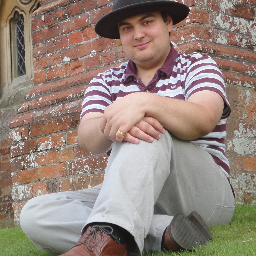
\includegraphics[width=0.32\textwidth]{mark.png}} &
  
\includegraphics[width=0.23\textwidth]{python.png}
\end{tabular}
\fbox{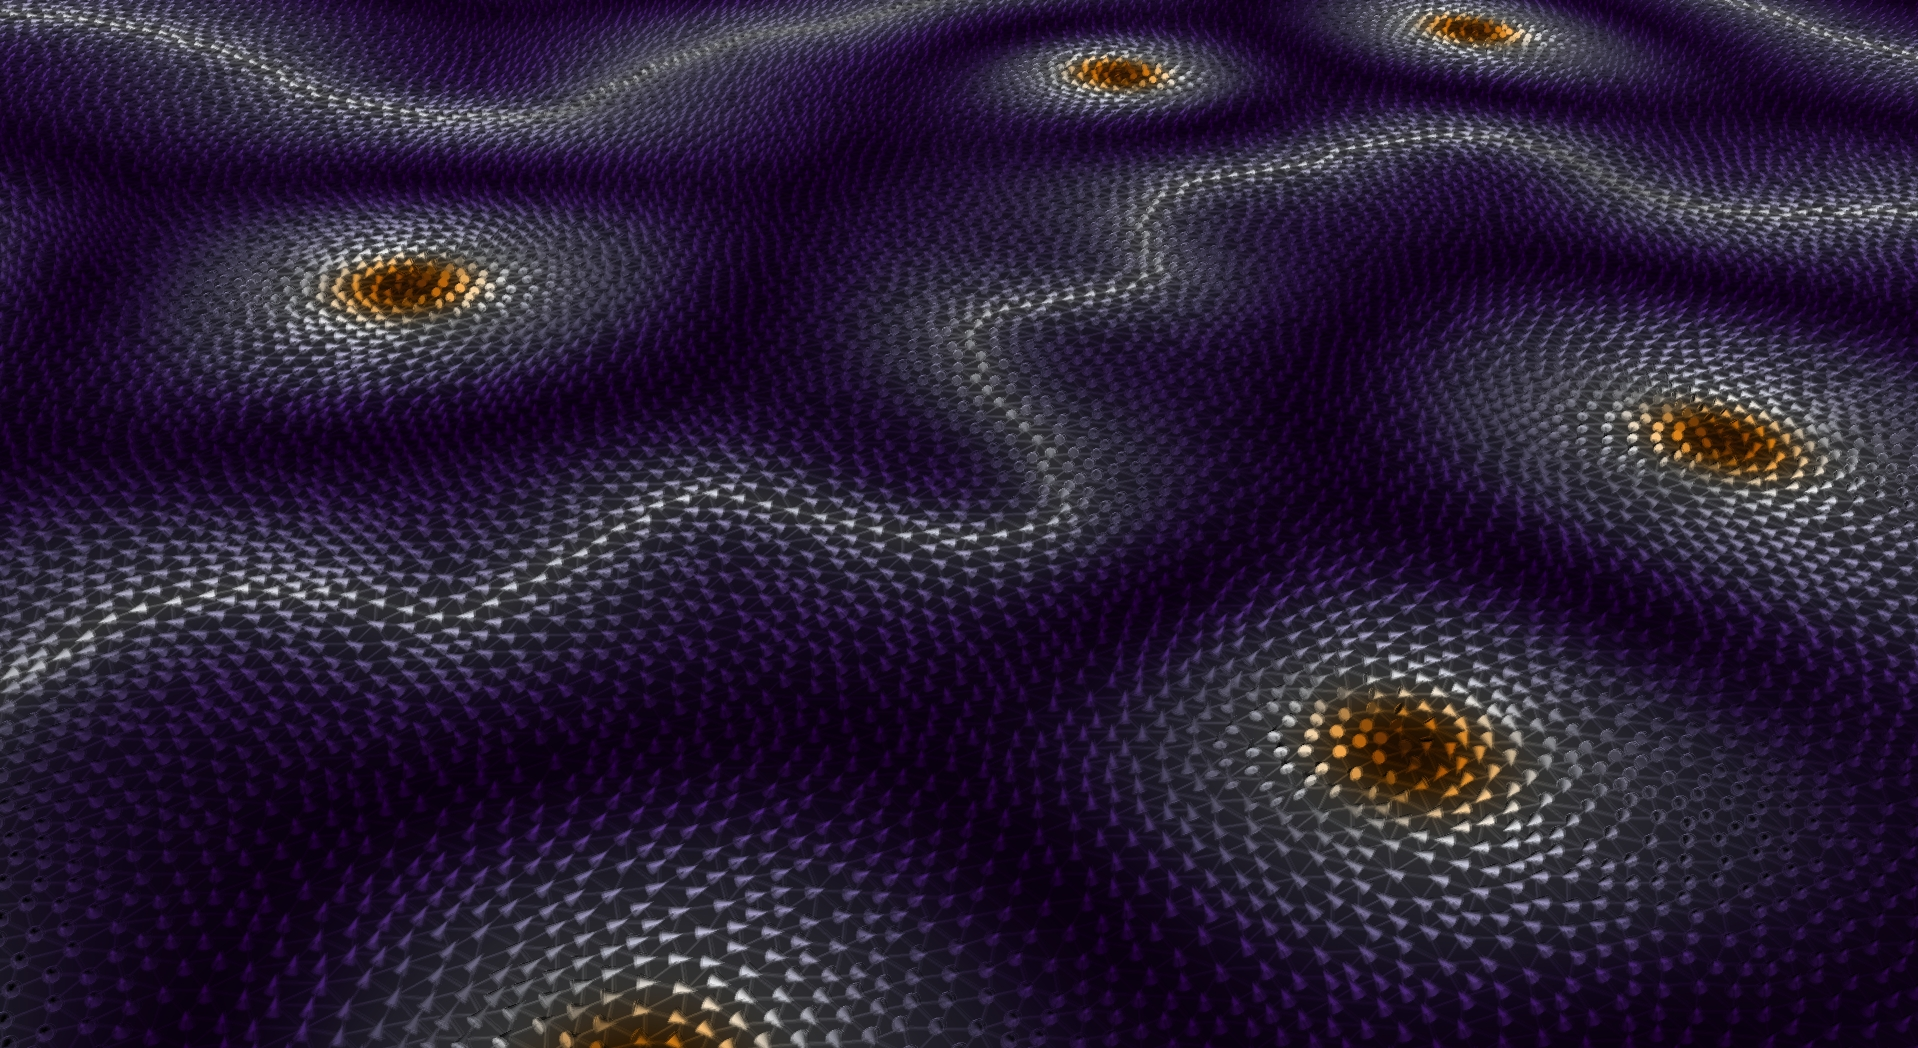
\includegraphics[width=0.6\textwidth]{hpc.png}}
\end{center}
\clearpage

\slidetitle{Why write tests?}
\begin{itemize}
\item Shows your software is fit for purpose
\item Do changes compromise your software?
\item Confidence!
\item Others can develop without risk
\end{itemize}
\clearpage

\slidetitle{Why {\color{red}not} write tests?}
\begin{itemize}[itemsep=-2.9pt]
\item Shows your software is fit for purpose
{\color{red} \item[\label={}] \hfill ``But I know it works!''}
\item Do changes compromise your software?
{\color{red} \item[\label={}] \hfill Takes time and skill}
\item Confidence!
{\color{red} \item[\label={}] \hfill False confidence!}
% Tests done badly are worse than no tests at all
\item Others can develop without risk
{\color{red} \item[\label={}] \hfill Increased codebase (more to maintain)}
\end{itemize}
\clearpage

\thispagestyle{empty}
\topskip0pt
\vspace*{\fill}
\LARGE{\centerline{Tests done badly are}
\centerline{worse than no tests at all.}}
\vspace*{\fill}
\clearpage

\end{document}
